\documentclass[a4paper]{jpconf}
\usepackage[utf8]{inputenc}
\usepackage{graphicx}
\usepackage{listings}
\usepackage{fancyvrb}

\providecommand{\keywords}[1]{\qquad\textbf{Keywords---} #1}
\begin{document}
\title{Recording the LHCb data and software dependencies }


\author{Ana Trisovic$^{1,2}$, Ben Couturier$^1$, Val Gibson$^2$ and  Chris Jones$^2$  }
\address{$^1$ CERN, Geneva, Switzerland}
\address{$^2$ University of Cambridge, Cambridge, the United Kingdom}
\ead{ana.trisovic@cern.ch}

\begin{abstract}In recent years awareness of the importance of preserving the experimental data and scientific software at CERN has been rising. To support this effort, we are presenting a novel approach to structure dependencies of the LHCb data and software to make it more accessible in the long-term future. In this paper, we detail the implementation of a graph database of these dependencies. We list the implications that can be deduced from the graph mining (such as a search for the legacy software), with emphasis on data preservation. Furthermore, we introduce a methodology of recreating the LHCb data, thus supporting reproducible research and data stewardship. Finally, we describe how this information is made available to the users on a web portal that promotes data and analysis preservation and good practise with analysis documentation.
\end{abstract}
%\keywords{data preservation, data provenance, graph database}

{
%\setlength{\parindent}{4em}
%\setlength{\parskip}{0.5em}

\section{Introduction}

The Large Hadron Collider beauty (LHCb) experiment at CERN is a general purpose detector in the forward region, which focuses on investigating the differences between matter and antimatter by studying the decays of beauty (\emph{B}) and charm (\emph{D}) mesons. The detector has been recording data from proton-proton collisions since 2010 and is expected to record data throughout the 2020s. Due to the rapid development of both the hardware and software used to process the data, many questions have been raised about data compatibility and preservation. In response to this, we are creating a database to record the metadata of our software and the data provenance. The recorded dependencies are expected to ease the process of running the software and analysing the data in the long-term future.

\subsection {Data preservation initiative}

 The data preservation project in High Energy Physics (HEP) aims to ensure the preservation of experimental and simulated data, as well as the scientific software and documentation. The main objective is to assist analysing HEP data in the future. The major use cases include looking for signals predicted by new theories and improving current measurements, in addition to physics outreach and educational purposes.

The LHCb data is processed with software and hardware that are changing over time. The information about the data, software and the changes have been logged in the internal databases and web portals. Our goal was to collect and structure this information into a singular, robust database that can be used immediately for scientific purposes and for the long-term future preservation. 

Finally, in support of making the LHCb data replicable and reusable, we concentrate our efforts to provide complete information on the data provenance and, to some extent, assist in its recreation independently of the CERN infrastructure.


\section{Overview of the LHCb software and data production}

The LHCb data production consists of the recording of the data by the LHCb detector, the processing of this data, and finally making the data available to physicists. In HEP analyses we also use the result of Monte Carlo simulations, which represent simulations of particle collisions. It is commonly used to help to characterize the signal (particle decay) of interest. These samples are kept in the same data format as the experimental (real) data and handled with the same software. In this paper, the term \emph{data} will be used to refer to both simulated data and the real experimental data.

The LHCb software is based on the Gaudi framework~\cite{barrand2001gaudi}. Gaudi is an object-oriented framework designed to provide a common infrastructure and environment for the different software applications of the LHCb experiment~\cite{corti2006software}. It is a modular software, which supports event data processing in real time inside the experiment, the data production in the offline system and the physics analyses performed by the users.

In each stage of the data production, we use a specialised software application. There are a number of versions of each application, in some cases over 100 different versions to date. Different versions can produce different physics output, thus making our data and physics results biased. Therefore it is crucial to know how the application manipulates the data in use. 


Initial stages of the Monte Carlo production~\cite{corti2015monte}:
\begin{itemize}
    \item \textbf{Simulation - Event generation.} The application {\it Gauss} mimics what happens inside the spectrometer of the LHCb experiment, simulating the initial data set of particle collisions~\cite{corti2006software}.
    \item \textbf{Digitization - Detector response.} The application {\it Boole} performs the simulation of the detector responses to produce the output in the same form as the experiment's electronics. 
    \item \textbf{L0 trigger emulation and  High level trigger (HLT).} Only a small fraction of the events produced in the LHCb detector are interesting to analyse. The trigger is a mechanism to select these events and save them, discarding the rest of the data (around 99\% of what was produced). The application that runs the triggers is {\it Moore}. Moore filters the simulated data in the same way as real data. 
\end{itemize}

The final stages in data production are the same for Monte Carlo samples as for the real data obtained by the data acquisition (DAQ) system (shown in Figures  \ref{fig:real} and \ref{fig:sim}). The settings in the applications are equivalent for both real data and simulation, to keep one consistent with the other:

\begin{itemize}
    \item \textbf{Turbo.} Turbo is a new streaming strategy where events are reconstructed in the trigger, thus bypassing the offline reconstruction and discarding the raw events~\cite{benson2015lhcb}. The application used in turbo stream, {\it Tesla}, writes out a compact summary of physics objects containing all the information necessary for analyses. 
    \item \textbf{Reconstruction.} In this stage, the detector hits are transformed into physics objects and written to disk. The {\it Brunel} application integrates the complete pattern recognition and produces files containing all reconstructed items such as calorimeter and trackers clusters, charged tracks and information on particle identification.
    \item \textbf{Streaming.} Streaming is the final stage of the production, which covers selection of the events. This is done with the {\it DaVinci} application~\cite{corti2006software}. \iffalse DaVinci is also used by the users doing analyses Hence, the output of the application can be purely statistical or event data. \fi
\end{itemize}


\iffalse 
\subsection{LHCb data production}

The experimental data is being recoded inside the LHCb detector. The expected detector output is obtained by computer simulation. We need the simulated data for the identification of particles and prediction of the detector behaviour. This data are often called Monte Carlo data. Both the experimental and simulated data go through the same production pipeline after they were created ~\cite{corti2006software}.

The data production pipeline is designed to maximise the data-taking efficiency and data quality. The pipeline consists of the following stages (figure 1), and at the each stage the input data is the product of the previous stage:

\begin{itemize}
    \item \textbf{Filtering data through the triggers.} This stage occurs while the data is being recorded inside the LHCb. Only a small fraction of the collisions inside the LHCb contain $B$ hadrons, and even a smaller fraction have interesting decays to study. If the triggers detect these decays, they will pass the data through, otherwise they will delete it. After selection in the fast hardware trigger, the data goes into the software triggers.
    \item \textbf{Reconstruction.} In this stage the detector hits are being transformed into objects such as particle tracks and clusters. The track fit determines the best estimate of the track parameters along the particle trajectory. We can obtain the momentum of the particle, position, direction etc. These objects are stored into an output file on disk.
    \item \textbf{Stripping.} The data is further filtered through a set of selections and more sophisticated track fits. This process reduces its size and makes it suitable and accessible to the users.
    \item \textbf{Users' analyses.} The users make their own cuts to the data and analyse it using their code.
\end{itemize}

\fi 
Figure \ref{fig:real} shows the real data production pipeline. After data acquisition in the {\it Online} system, the data is stored in RAW data format. It is further processed in \emph{Reconstruction} and \emph{Streaming} or \emph{Turbo} stages, before it is stored on a disk and made available to the physicists. 
Figure \ref{fig:sim} shows Monte Carlo simulation pipeline. The dice in the beginning of the pipeline represent a random generator, that is a central part of the simulation generation. The names of stages are followed by the names of applications used in each stage. 

\begin{figure}[h]
    \centering
    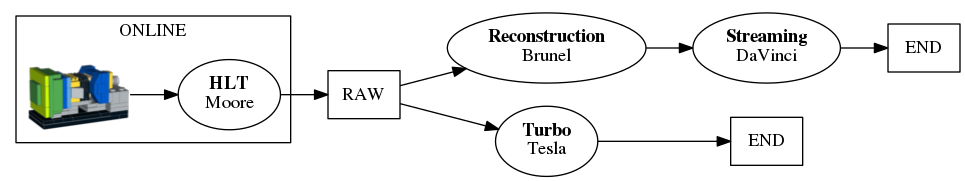
\includegraphics[width=\textwidth]{img/real}
    \caption{The real data production pipeline}
    \label{fig:real}
\end{figure}

\begin{figure}[h]
    \centering
    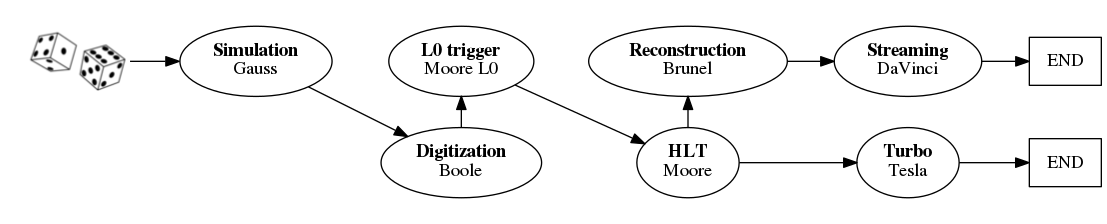
\includegraphics[width=\textwidth]{img/sim2}
    \caption{The simulation production pipeline}
    \label{fig:sim}
\end{figure}

\iffalse
\subsection{LHCb software stack}

The LHCb software stack is based on Gaudi framework~\cite{barrand2001gaudi}. It is modular software, which supports event data processing applications that run in real time high level triggers, the data and Monte Carlo production in the offline system and the physics analysis preformed by the users.

There are specialised software applications that are used in each of the stages. In some stages, such as creating simulated data, we use two different applications in the process. Different versions of an application can produce very different physics output, therefore it's crucial to know how the application manipulates the data in use. There are numerous versions of each of the applications, some of them reaching over 100 different versions.
\fi


\section{Implementation}

\subsection{The database design and technologies}

For the storage implementation we chose a graph database, as it provides flexibility in object dependencies that relational databases cannot capture. Firstly, the modules in the LHCb software are connected in a complex way that can be elegantly presented in a graph. Secondly, by adopting a graph database approach, we are able to accommodate the changes that come with time and the new LHC run standards. For instance, we can easily add to the nodes a new attribute for \emph{data quality}, even though they were not there originally.

A graph database is a storage engine that stores data as nodes and relationships and allows high performance retrieval and querying of those structures. Properties can be added to both nodes and relationships. One of the most prominent graph databases, and the technology used in our solution, is \emph{Neo4j}\footnote{Official web page of the Neo4j technology: https://neo4j.com/}. It is an open source NOSQL graph database implemented in Java. Objects in \emph{Neo4j} are manipulated with the \emph{CYPHER} query language, which is SQL-inspired, declarative and can describe patterns in graphs using an ascii-art syntax.


Our database implements the following nodes:
\begin{itemize}
    \item {\bf{Production.}}
    A production node captures a list of steps which define the LHCb data production pipeline. There are three types of \emph{Production} nodes, and those are: simulation models (prerequisite for simulation production), simulation and real data production. 
    
    Every node is described with a list of attributes (as shown below in JSON). The \emph{Name} value includes the year of data-taking (here 2016), beam energy and the kind of collision, in this case that is \emph{Proton-Argon}. At LHCb we mostly examine proton-proton collisions, but also proton-helium, proton-neon etc. {\it ID} stands for the identification number of the production and {\it DQflag} is a data quality flag. Every step has its own ID number and a list of configuration tags, such as {\it DDDB} and {\it CondDB} tags which define detector and conditions respectively, python \emph{Options} file and \emph{Input} and \emph{Output} data formats.
    
    \begin{Verbatim}[numbers=left,xleftmargin=5mm]
{
  "ID": "31034",
  "Name": "Reco16-Beam2510GeV-MagDown-ProtonArgon",
  "Type": "Reconstruction",
  "EventType": "90000000 Full stream",
  "ProcessingPass": "Real Data",
  "DQflag": "OK",
  "Step": [
    {
      "ID": "129609",
      "Application": "Brunel-v50r1",
      "System_config": "x86_64-slc6-gcc49-opt",
      "Options": "$APPCONFIGOPTS/Brunel/DataType-2015.py;$APPCONF...",
      "DDDB": "dddb-20150724",
      "CondDB": "cond-20160517",
      "Extra": "AppConfig.v3r272",
      "Input": "RAW(Y)",
      "Output": "BRUNELHIST(Y),FULL.DST(Y)"
    },
    { ... }
  ]
}
    \end{Verbatim}
    \item {\bf{Project.}}
    A project describes one version of a module in the LHCb software stack. The class is defined with a project name and version, for example \emph{BRUNEL v44r8} or \emph{DAVINCI v36r2}. The projects are built depending on each other, and each project version requires specific set of other projects to run. To demonstrate this {\it REQUIRES} relationship, below is the \emph{CYPHER} code that finds a path \textbf{\emph{p}} from an application in the top level of the LHCb software stack DaVinci, to the Gaudi framework, which is the base of the stack. The result of this query is a path which normally contains several nodes and includes all the projects that are required to run the DaVinci application.

\begin{verbatim}
MATCH   p = (a:Application{project:’DAVINCI’})-
            [r:REQUIRES*..]->
            (d:Framework{project:’GAUDI’})
            RETURN p LIMIT 1
\end{verbatim}

An example of the output of the previous query is:

\begin{lstlisting}[
  mathescape,
  columns=fullflexible,
  basicstyle=\fontfamily{lmvtt}\selectfont,
]
DAVINCI v33r1 $\to$ ANALYSIS v10r3 $\to$ PHYS v16r3 $\to$ REC v14r3 
$\to$ LHCB v35r3 $\to$ GAUDI v23r5
\end{lstlisting}
    
    \item {\bf{Platform.}}
    A platform describes a computer environment that supports the LHCb software. For instance, \verb|x86_64-slc6-gcc49-opt| means optimized (opt) \verb|x86_64| architecture of Scientific Linux CERN 6, and conventionally gcc49 stands for GNU Compiler Collection (GCC). Links between \emph{Projects} and \emph{Platforms} define compatible platforms for each project. For example, a list of compatible platforms for \emph{DAVINCI v38r0} is shown in the table below.
    
    \begin{center}
    \begin{tabular}{ l l }
    Project & Platform \\
    DAVINCI v38r0 & \verb|x86_64-slc6-gcc49-opt| \\
     & \verb|x86_64-slc6-gcc48-opt| \\
     & \verb|x86_64-slc6-gcc48-do0| \\
     & \verb|x86_64-slc6-gcc49-dbg| \\
     & \verb|x86_64-slc6-gcc48-dbg| \\
    \end{tabular}
    \end{center}

\end{itemize}
\par{
Object-Relational Mapping (ORM) in computer science is a programming technique for querying and manipulating data from a database using an object-oriented paradigm. For each node label in the graph database (\emph{Production, Project, Platform}), there is a corresponding Python class, which enables the use of the objects from within the programming language. The ORM used in this project is called {\it neomodel}\footnote{More about {\it neomodel} can be found on GitHub: https://github.com/robinedwards/neomodel} and it is specific for the \emph{Neo4j} graph database.}
\par {An example to illustrate the schema of the database is shown in Figure \ref{fig:str}.}
    
    \begin{figure}[h]
    \centering
    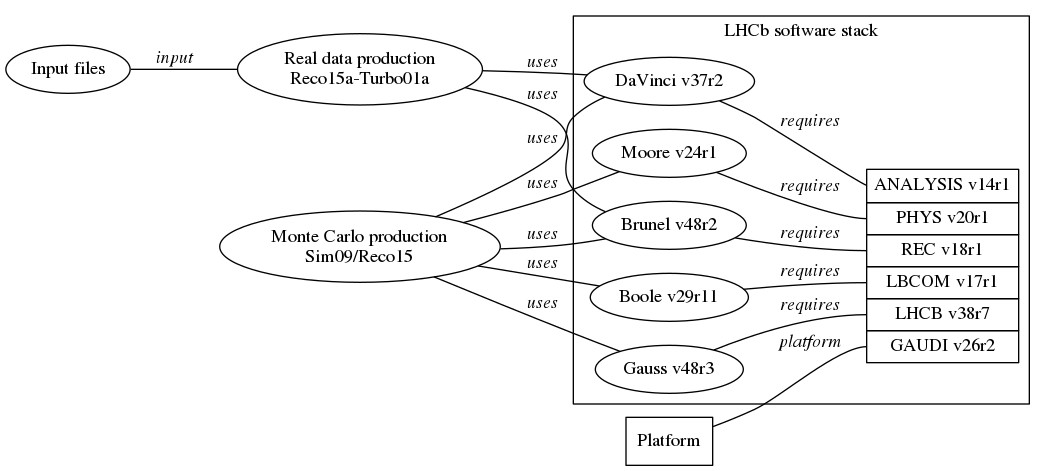
\includegraphics[width=\textwidth]{img/dbstruct}
    \caption{The graph database schema. }
    \label{fig:str}
    \end{figure}
    


\subsection{Application Programming Interface API}

The API to the LHCb graph database is implemented in \emph{py2neo} which is a client library and toolkit for working with \emph{Neo4j} from within Python applications and from the command line. We use the Representational State Transfer (REST)~\cite{jakl2005representational} architectural style to create a request/response mechanism between the server and the client. The data retrieved directly from the database is returned in JSON format. Some of the functions are listed below:

\begin{itemize}
    \item {\bf{ \verb|getProductionSequence(ID)|}} Returns a \emph{Production} entity with the given \emph{ID} number.
    \item {\bf{ \verb|listProjects()|}} Returns the list of \emph{Projects}.
    \item {\bf{ \verb|listPlatforms(Project)|}} Lists the suitable \emph{Platforms} for the given \emph{Project}.
    \item {\bf{ \verb|listRequirements(Project)|}} Lists the required modules for the given \emph{Project}.
\end{itemize}

\subsection{Web portal}

The graph database is connected to a \emph{Django} web server and made available for the users as a web portal. Django is a high-level, open source Python Web framework that encourages clean and pragmatic design of the web applications~\cite{holovaty2009definitive}.

The web portal allows browsing through the LHCb data production and software information. It implements a search engine for this metadata, and it is meant to recommend the latest streaming to the users. In addition, it should promote the LHCb data preservation and provide a comprehensive user guide for analysis documentation and preservation.

\iffalse
\begin{figure}[h]
    \centering
    \includegraphics[width=0.9\textwidth]{img/slide1}
    \caption{Appearance of the web page}
    \label{fig:webp}
\end{figure}
\fi


\section{Functionality}

\subsection{Methodology for preservation and recreation}

The instances of the class {\it Production} consist of a sequence of steps, where every {\it Step} provides complete configuration information to rerun one stage in the data production. This configuration information is easily transformed into a \emph{Python file} that can be run in the LHCb computing environment, thus producing the data. However, the production can be run outside the CERN infrastructure, making the LHCb data replicable and sustainable for the long-term future. Next to the configuration information, other requirements include:
\begin{itemize}
    \item {\bf Software from CERN Virtual Machine File system (CVMFS)\footnote{Official web page of CERN VMFS: https://cernvm.cern.ch/portal/filesystem}.} CVMFS is an open  source file system designed for efficient software distribution~\cite{buncic2010cernvm}. The HEP experiments install all released software components in its final configuration on CVMFS~\cite{shiers2016cern}. 
    \item {\bf Computing environment.} The LHCb software is developed for the Linux operating system, specifically Scientific Linux CERN 5 or 6 (slc5 or slc6 respectively). If these distributions are unavailable, it is necessary to mount an image on virtual machine or container engine such as \emph{Docker}\footnote{Official web page of the Docker technology: https://www.docker.com/} to run Linux and the LHCb computing environment from CVMFS.
    \item {\bf Input files (RAW).} In real data processing, input files created at the LHCb detector are required. These files need to be stored in such way to be accessible from within the application. In Monte Carlo production, input files are not required as all the events are simulated inside the application.
\end{itemize}

% The procedures for building, installing and validating software releases remains under the control  and responsibility of each user  community.  We  provide  a  mechanism  to  publish  pre-built  and  configured  experiment software  releases  to  a  central  distribution  point  from  where  it  finds  its  way  to  the  running CernVM  instances  via  the  hierarchy  of  proxy  servers  or  content  delivery  networks.
%Future work will include preserving the LHCb workflows and methods. We will assist sharing, publishing and preserving of our workflows.

\subsection{Recording data provenance}

Data provenance has evolved to be an integral part of best practise for long-term data preservation and research reproducibility. It certifies the origin of the data, and in computational terminology it is defined as the representation of the relationship between data items (\emph{entities}), transformations (\emph{activities}), and individuals or organisations (\emph{agents}) in a graph. These graphs capture when, by whom and how a data item was created and/or processed. Provenance systems typically concern some aspects of: data quality, replication recipes, ownership attribution, context understanding and audit~\cite{simmhan2005survey}.

The LHCb graph database records the data provenance by explicitly linking the raw data sets to processing sequence they went through. It mostly follows the typical structure, except for the absence of the executor, as the activities are organized by the LHCb experiment collaboration. The LHCb software is open source and available on GitLab\footnote{GitLab repository of the LHCb software: https://gitlab.cern.ch/lhcb-core}, which allows the users to independently track the computational performance. %To complete the  provenance, we aim to add the information about the dates of data-taking.

\subsection{Source for CERN Analysis Preservation portal}

\emph{The CERN Analysis Preservation (CAP)} portal is a joint project across the LHC experiments at CERN~\cite{dallmeiercern}. They manage the computing resources and a portal for analysis preservation. The aim is to promote good practise in performing physics analysis and assist in analysis preservation and reproducibility. 

On the web portal, analyses should be documented in a form completed by the authors. The portal can query the working group databases and the graph database to get some of the information needed in the form. The form sends a REST request with parameters and the server returns required information in JSON. Currently, the API provides the application used in a given production, and platform information for each application.

\subsection{Graph mining}

Graph mining is the process of finding and extracting concealed information from graphs. This information can be worthwhile for the future project management and the community, particularly for the long-term preservation activities. The information that we can easily extract from the LHCb graph database are:
\begin{itemize}
    \item {\bf The most used project versions.} The \emph{Project} nodes with the highest degree in the graph are the most used versions. They are likely to be often reused in future and should be preserved having this in mind.
    \item {\bf Obsolete project versions.} On the contrary, we can identify obsolete software versions as the \emph{Project} nodes with the lowest degree. This information is valuable because we can archive and remove them in a new release of CVMFS.
    \item {\bf Project classification.} We can classify the projects into groups where each of them run with a specific subset of the data (eg. 2011 data). This is particularly important for testing the projects against their corresponding data sets and verifying they work in the same way in the future as they work today.
    \item {\bf Troubleshooting.} Identifying the data sets handled by a faulty software component. Given that there is a defect in one of the projects, we can search through the graph to find the affected data sets.
\end{itemize}

\subsection{Other use-cases}

The graph database is regularly used in the LHCb software production, providing the information on project (module) dependencies and the order in which they should be built. Other use-cases include: recommending the latest streaming, searching and browsing through the LHCb software and data tags, finding all the modules required by a project and vice versa, finding the modules supported by a project, eg. what project are run on top of \emph{GAUDI vXrY}. This functionality is provided to the users at the web portal.


\section {Conclusion}


In this paper we presented the LHCb graph database, a novel approach for recording dependencies between the software and data. The data nodes in the graph represent each production of experimental or simulated data, while the software nodes represent each project within LHCb, how it depends on other projects (modules) and how it is linked to the data production. Furthermore, we introduced a methodology to recreate a data set independently of the CERN computing infrastructure using the information stored in the \emph{Production} nodes. We are concentrating our efforts to advance this methodology to make the LHCb data replicable, reusable and sustainable for the long-term preservation.  

\section *{Acknowledgements}

The authors would like to thank Marco Cattaneo and Gloria Corti for providing inside information about the data and simulation production at LHCb. We are grateful for their constructive suggestions for the data preservation initiative and for answering our questions. Thank you to Philippe Charpentier, Federico Stagni and Zoltan Mathe for answering our questions about LHCb Bookkeeping and Dirac. Special thanks to Vladimir Gligorov and Agnieszka Dziurda for following this project and providing their insights and ideas. Thank you to Silvia Amerio for suggesting various use-cases. Thank you to Illya Shapoval for starting off the use of Neo4j at LHCb.


\section*{References}
\bibliographystyle{iopart-num}
\bibliography{ref}
}


\end{document}


